% WikiHow-MY: instructional English->Myanmar MT corpus + IFS metric.
% Official ACL style (acl.sty + acl_natbib.bst from github.com/acl-org/acl-style-files).
% Build: pdflatex main; bibtex main; pdflatex main; pdflatex main.
% [review] => anonymized + line numbers for double-blind submission. For camera-ready,
%   switch to \usepackage[final]{acl} and uncomment the author block below.
% Numbers are traceable to experiments/results/*.json via \input{tables/*}.
\documentclass[11pt]{article}
\usepackage[final]{acl}
\usepackage{times}
\usepackage{latexsym}
\usepackage[T1]{fontenc}
\usepackage[utf8]{inputenc}
\usepackage{microtype}
\usepackage{booktabs}
\usepackage{graphicx}

\title{WikiHow-MY: A Human Post-Edited English--Myanmar Instructional MT Corpus
and an Instruction-Faithfulness Score for Procedural Translation}
\author{Anonymous (WMT 2026 submission)}
% === CAMERA-READY AUTHOR BLOCK — uncomment for the de-anonymized version. ===
% KEEP the anonymous \author above for double-blind WMT/ACL review: a name or any of
% the resource links below in the SUBMITTED pdf de-anonymizes the author -> desk reject.
% \author{Pyae Sone Kyaw \\ Independent Researcher \\ \texttt{pyaesonekyaw1022000@gmail.com}}
% Resource links to add to the Release/Availability paragraph at camera-ready (all withheld for review):
%   Model:      https://huggingface.co/PyaeSoneK/nllb-600m-wikihow-en-my
%   Collection: https://huggingface.co/collections/PyaeSoneK/english-to-burmese-mt-wikihow-6a28b3f136f02ab48e0d62c4
%   Code:       https://github.com/soneeee22000/wikihow-mt-my  (public; rehydration only, does NOT mirror English source)
%   Kaggle (reproducibility; set each notebook Public before camera-ready, else 403):
%     train:  https://www.kaggle.com/code/pyaesonekyaw/wikihow-my-ft
%     eval:   https://www.kaggle.com/code/pyaesonekyaw/wikihow-metricx-run
%     rerank: https://www.kaggle.com/code/pyaesonekyaw/wikihow-nbest-run
\date{}

\begin{document}
\maketitle

\begin{abstract}
We present \textbf{WikiHow-MY}, to our knowledge the first instructional/how-to
English--Myanmar parallel corpus: $\sim$10k human post-edited (MTPE), quality-checked
sentence pairs from WikiHow, released by rehydration under CC BY-NC-SA 3.0 with
article-disjoint splits. On this resource we benchmark NLLB-200 (zero-shot and
fine-tuned), Google Translate, and Gemini 2.5 with chrF++/spBLEU/BLEU/COMET, and find
that \emph{surface and semantic metrics disagree on the best system}. We then introduce
the \textbf{Instruction Faithfulness Score (IFS)}, an interpretable, source-anchored
metric that decomposes procedural fidelity into step, action, entity, and quantity
preservation---the strongest hand-checkable proxy for procedural fidelity we can
construct---and use it as a diagnostic in the first human \emph{instruction-followability}
study for a low-resource language (9 raters, 420 ratings), where learned metrics such as
COMET are known to be poorly calibrated. The finding generalizes beyond any single metric:
\emph{none} of the metrics we test---surface (chrF++/BLEU) or our procedural IFS---is correlated
with human followability at the segment level ($r{\approx}0$), and surface-saturating metrics,
IFS included, \emph{cannot rank systems}: IFS spans just 2.25 points across the four systems,
awards its highest score to the fine-tuned model humans place third of four, and ranks humans'
best system only third. We then show this is a failure of \emph{estimation}, not of measurability:
keeping IFS's four procedural dimensions but estimating them with a learned per-dimension judge
rather than surface preservation recovers human followability ($r{=}0.53$ vs.\ $0.13$) and the
system ranking (Spearman $1.00$ vs.\ $0.20$), including when the judge's own outputs are held
out. Our contribution is thus both a diagnostic \emph{when-metrics-fail} result for procedural
MT---followability is not recoverable from surface, source-anchored preservation---and its
constructive counterpart: it \emph{is} recoverable when those same dimensions are estimated per
dimension by judgment.
Finally, we probe whether decoding-time reranking can close the in-domain gap to the
commercial system, and report a negative result: although a reference-optimal selection
from the fine-tuned model's $n$-best \emph{beats} Google Translate, no reference-free
signal---learned quality estimation, structural IFS, or MBR---recovers this gain, a
concrete decoding-time symptom of learned-metric miscalibration for Burmese.
\end{abstract}

\section{Introduction}
Procedural, instructional text---how-to guides, recipes, manuals---is high-stakes to
translate: a reordered step, a dropped negation, or an altered quantity can make the
instructions \emph{unfollowable}, a failure mode standard MT evaluation does not isolate.
This problem is acute for low-resource languages such as Burmese (Myanmar), where parallel
data is scarce and existing resources are news-domain (ALT, \citealp{alt2016}) or
web-crawled (NLLB, \citealp{nllb2024}); the WikiHow-derived multilingual resource
WikiLingua \citep{wikilingua2020} does not include Burmese.

We make four contributions:
(1) \textbf{WikiHow-MY}, the first instructional English--Myanmar MTPE corpus
(\S\ref{sec:corpus});
(2) a \textbf{benchmark} of open, commercial, and LLM systems showing that surface
(chrF++/spBLEU) and semantic (COMET) metrics rank the systems differently (\S\ref{sec:bench});
(3) the \textbf{Instruction Faithfulness Score (IFS)}, a procedural-fidelity metric for MT,
together with a human-followability study (\S\ref{sec:human}) showing that its automatic form---
like chrF++ and BLEU---fails to track followability and, being range-restricted, carries no
usable system-ranking signal, a
\emph{when-metrics-fail} result for a setting where learned metrics are also miscalibrated
\citep{falcao2024comet,africomet2024} (\S\ref{sec:ifs});
and (4) a constructive counterpart: keeping those four dimensions but estimating them with a
\textbf{learned per-dimension judge} instead of surface preservation recovers both segment-level
followability ($r{=}0.53$ vs.\ $0.13$) and the system ranking ($\rho{=}1.00$ vs.\ $0.20$),
on held-out systems too (\S\ref{sec:estimator}).
We additionally probe decoding-time reranking and report a negative result: the gain
needed to match the commercial system is present in the fine-tuned model's $n$-best but
unreachable by any reference-free selector (\S\ref{sec:rerank}).

\paragraph{Scope clarification.} ``Instruction-followability'' here is a property of a
\emph{translation} (can a reader execute the procedure from the target text?), distinct
from ``instruction-following'' in the LLM sense of a model obeying a prompt
\citep{ifeval2023,xifbench2025}. It is likewise distinct from translation
\emph{instruction-following} benchmarks \citep{ifmtbench2026}, which test whether an MT system
obeys author-supplied constraints (format, terminology, register); we ask instead whether the
resulting translation lets an end user carry out the procedure. We operationalize this as
task-based MT evaluation \citep{gale_taskbased} in the functionalist/skopos tradition
\citep{reissvermeer1984}.

\section{Related Work}
\paragraph{Low-resource and Burmese MT.} NLLB-200 \citep{nllb2024} is the standard open
baseline, evaluated on FLORES-200/+ \citep{flores200,floresplus2024}; ALT \citep{alt2016}
is the de-facto en--my (news) set; BURMESE-SAN \citep{burmesesan2026} is the most recent
Burmese LLM benchmark and scores MT with MetricX-24 \citep{metricx2024} on FLORES+.
Burmese is written without word boundaries and historically split between Zawgyi and
Unicode encodings, motivating character-level metrics (chrF++, \citealp{chrfpp2017}) and
SentencePiece-based spBLEU \citep{flores101spbleu2022} over tokenizer-dependent BLEU
\citep{bleu2002}.

\paragraph{MT metrics and faithfulness.} Beyond surface metrics, learned metrics
COMET \citep{comet2020} and MetricX-24 \citep{metricx2024} lead segment-level correlation
but are documented to be unreliable for low-resource languages
\citep{falcao2024comet,africomet2024}. Entity- and number-preservation are established
evaluation targets---WMT Critical Error Detection NUM/NAM \citep{wmtced2022}, manual entity
accuracy M-ETA \citep{meta2024}, challenge sets ACES \citep{aces2022}, and behavioural numeral
testing \citep{wang2021numerals}---so IFS \emph{adopts} (and cites), rather than claims, those
two components. Procedural-correctness
metrics (action precision, step edit-distance, ingredient/quantity preservation) appear in
recipe \emph{generation} \citep{recipegen2025}---we \emph{adapt} these signals rather than
invent them. Decomposed \emph{reference-free} MT evaluation is itself not new either, existing
along generic MQM dimensions \citep{park2024multidim}; but we are, to our knowledge, the first to
operationalize step-ordering and imperative-action preservation as a \emph{procedural} axis for
reference-free MT evaluation, and the first to validate an automatic procedural-fidelity MT
metric against human followability---the first such validation for a low-resource language. METEOR \citep{meteor2005} rewards
intra-sentence word order; IFS instead measures procedural \emph{step} order.

\paragraph{Procedural text and followability.} WikiHow encodes ordered, goal-directed steps
\citep{wikilingua2020}; functionalist translation theory \citep{reissvermeer1984} treats
instructions as ``operative'' texts judged by whether they elicit correct reader action,
and task-based MT evaluation \citep{gale_taskbased} measures whether a user can complete a
task from MT output. We synthesize these into a followability construct for procedural MT,
with error severity grounded in MQM \citep{mqm2021}.

\paragraph{Agentic MT (future work).} Reflection/refinement MT \citep{selfrefine2023,
ng2024transagent,tear2025,llmrefine2024} and metric-guided selection \citep{maps2024} use
generic quality signals (MQM/COMET); using a structured procedural-fidelity score as an
in-loop control signal is unexplored and is the subject of follow-on work (\S\ref{sec:concl}).

\section{The WikiHow-MY Corpus}\label{sec:corpus}
WikiHow-MY contains \textbf{10{,}056} English--Myanmar sentence pairs from \textbf{82}
WikiHow articles. Translations are \textbf{machine-translation post-edited (MTPE) and
quality-checked} by Myanmar native speakers---we do not claim gold-standard human
translation. English sentences average 14.3 tokens (median 13, p95 28); Myanmar sentences
average 93 characters (median 85). Myanmar text is normalized to Unicode (no Zawgyi rows
detected) following the encoding considerations above.

\paragraph{Splits.} We split \textbf{by article} (GroupShuffleSplit, seed 42) into
train/dev/test of \textbf{8{,}302 / 908 / 846} pairs with \textbf{zero shared articles}.
Article-disjoint splitting does not by itself preclude repeated boilerplate sentences across
splits, so we additionally audit sentence-level leakage: only 2 of 846 test sources also
occur in train (1 in dev), and \emph{zero} test (source, target) \emph{pairs} are shared with
train or dev---so no test target is memorisable from training. Because the Myanmar references
are newly produced by post-editing and were not previously public, the evaluation pairs likewise
cannot appear in any benchmarked system's pre-training data. Figure~\ref{fig:stats}
summarizes the distributions.

\paragraph{Provenance and reference bias.} The corpus combines a professionally post-edited
subset and a volunteer post-edited subset; the specific base MT engine used to seed
post-editing was not recorded by the original creators. Because post-edited references are an
exacerbated translationese that can favor the seeding system and inflate surface metrics
\citep{toral2019posteditese,freitag2020references,zhang2019translationese}, we explicitly test
for this bias rather than assume it away (\S\ref{sec:bench}): a segment-level analysis finds
no copy signature toward any benchmarked system, and an out-of-domain FLORES+ control shows
the residual reference effect, if anything, favors our \emph{fine-tuned} model (which learns
this corpus's post-edit style) rather than the commercial systems. We additionally report
learned, reference-light metrics (COMET, MetricX-24) that are less sensitive to reference
surface form.

\paragraph{Release.} To respect WikiHow's CC BY-NC-SA 3.0 license (pre-2025 content), we
release by \emph{rehydration}---Myanmar translations, source URLs/IDs, and a build script---
never mirroring the English source; the released data carries CC BY-NC-SA 3.0 with attribution.

\begin{figure}[t]
\centering
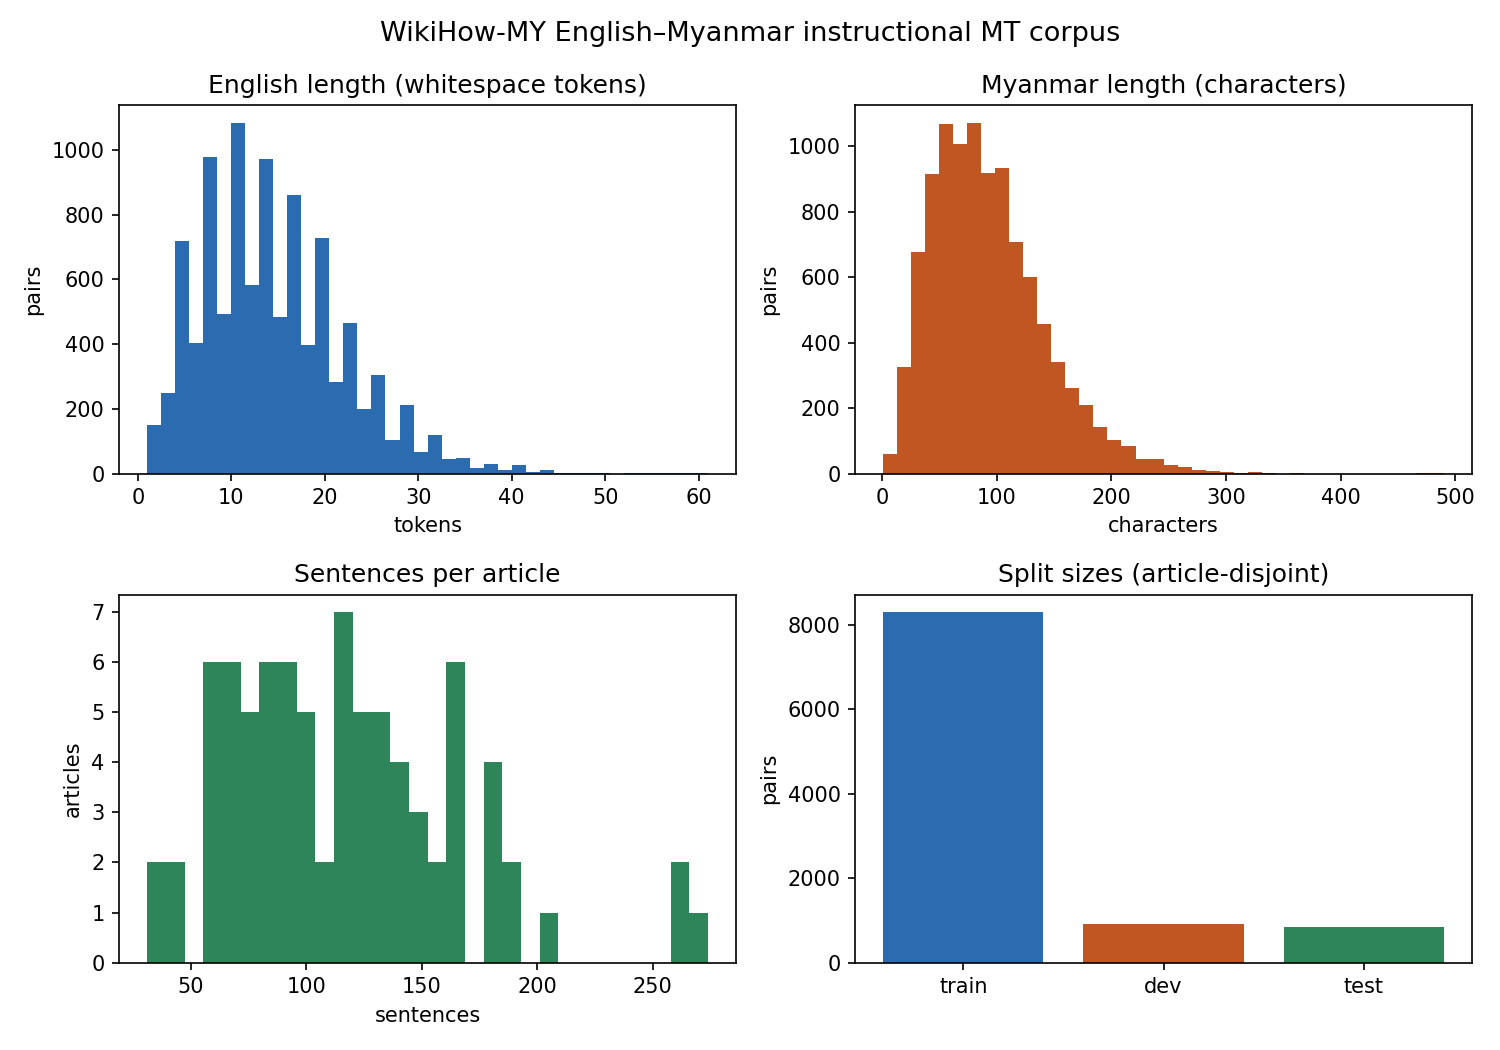
\includegraphics[width=\linewidth]{figures/dataset_stats.png}
\caption{WikiHow-MY corpus statistics (lengths, per-article distribution).}
\label{fig:stats}
\end{figure}

\section{Benchmark}\label{sec:bench}
We evaluate, English$\rightarrow$Myanmar, on the article-disjoint test set ($n{=}846$):
NLLB-200-distilled-600M zero-shot and fine-tuned (LR $3{\times}10^{-5}$, early-stopping on
dev chrF, seed 42), Google Translate (web), and Gemini 2.5 Flash (5-shot). We report chrF++
(primary; segmentation-agnostic for unsegmented Myanmar), spBLEU (FLORES-200 tokenizer),
tokenized BLEU, COMET (\texttt{wmt22-comet-da}), and MetricX-24
(\texttt{hybrid-xl-v2p6}, reference-based; an error score in $[0,25]$, lower is better)
\citep{metricx2024}---the learned metric used by BURMESE-SAN, included here for direct
comparability. All numbers are generated from JSON, not hand-typed.

% auto-generated by src/eval/make_tables.py -- do not edit by hand
\begin{table}[t]
\centering
\small
\begin{tabular}{lrrrrrr}
\toprule
System & chrF++ & spBLEU & BLEU & COMET & MetricX$\downarrow$ & IFS \\
\midrule
NLLB-200-distilled-600M (zero-shot) & 36.01 & 19.33 & 2.62 & 0.86 & 4.09 & 94.11 \\
NLLB-200-distilled-600M (fine-tuned) & 41.64 & 23.18 & 3.74 & 0.89 & 3.23 & 95.79 \\
Gemini 2.5 (5-shot) & 42.59 & 24.77 & 3.47 & 0.90 & 2.39 & 94.33 \\
Google Translate & 43.60 & 27.65 & 5.07 & 0.89 & 2.71 & 95.27 \\
\bottomrule
\end{tabular}
\caption{English$\rightarrow$Myanmar results on the WikiHow-MY test set (article-disjoint, $n$=846). chrF++ is the primary metric; spBLEU uses the FLORES-200 tokenizer; MetricX-24 (hybrid-XL, reference-based) is an error score in $[0,25]$ where lower is better ($\downarrow$); IFS is the Instruction Faithfulness Score.}
\label{tab:main}
\end{table}


\paragraph{Findings.} Fine-tuning improves substantially over zero-shot on every metric
(+5.6 chrF++; COMET $0.858\rightarrow0.886$; MetricX-24 $4.09\rightarrow3.23$).
However, \emph{surface and learned metrics disagree on the best system}: Google Translate
leads on all surface metrics (chrF++/spBLEU/BLEU), whereas \emph{both} learned metrics rank
Gemini~2.5 Flash first (COMET $0.904$; MetricX-24 $2.39$ vs.\ Google Translate's $2.71$).
That two independently trained learned metrics agree---and agree with BURMESE-SAN
\citep{burmesesan2026}, where Gemini-class models top MetricX---indicates the split is
genuinely surface-vs-semantic rather than a single-metric artifact. Yet learned metrics carry
their own documented low-resource miscalibration \citep{falcao2024comet,africomet2024} and are
opaque about \emph{what} they reward; this motivates an interpretable, procedure-aware metric.

\paragraph{Is the benchmark biased by post-edited references?} Because our references are
post-edited, a natural concern is that surface metrics favor whichever engine seeded the
post-editing (plausibly a commercial system). We test this two ways. First, a segment-level
copy analysis: if references were post-edited from system $X$, $X$'s raw output would
reproduce many references near-verbatim. It does not---exact-match rates against the reference
are uniformly near-zero (Google Translate $0.24\%$, Gemini $0.24\%$, fine-tuned NLLB
$0.47\%$), with Google Translate \emph{not} the leader and the few matches being trivially
short segments. Second, a domain-controlled comparison on FLORES+ (Table~\ref{tab:flores}),
whose references are independent professional translations, never post-edited from our systems
(and whose devtest is fully disjoint from our test set---zero shared source sentences or pairs).
Crucially, Google Translate's lead over fine-tuned NLLB \emph{widens} from $+2.0$ chrF++
in-domain to $+8.8$ on FLORES+. A reference bias favoring Google Translate would predict the
opposite (a larger in-domain gap); the actual pattern shows that the residual reference effect
favors our \emph{fine-tuned} model in-domain---it has learned this corpus's post-edit style---
so our WikiHow numbers are, if anything, generous to the open model rather than to the
commercial baseline. Finally, the surface-vs.-learned metric disagreement we observe
in-domain (surface metrics rank Google Translate first, while COMET and MetricX-24 rank
Gemini first) reproduces on the independent FLORES+ references---where Gemini again leads on
both learned metrics (MetricX-24 $3.08$ vs.\ $3.31$)---confirming it is a property of the
metrics, not an artifact of our post-edited references.

\paragraph{Domain generalization (FLORES+).} The same FLORES+ evaluation doubles as a
generalization check. Fine-tuning improves \emph{both} domains and \emph{all} three metrics
---in-domain $+5.6$ chrF++ / MetricX-24 $4.09\rightarrow3.23$, and out-of-domain $+4.3$ chrF++
/ MetricX-24 $5.64\rightarrow4.80$---so adapting to WikiHow yields no catastrophic forgetting
on general-domain text. As expected, absolute scores are weaker on FLORES+ (broad-domain,
longer sentences); the large out-of-domain gap to Google Translate also shows that our gains
are domain-specific, motivating in-domain enhancement rather than claims of general parity.

% auto-generated by src/eval/make_tables.py -- do not edit by hand
\begin{table*}[t]
\centering
\small
\begin{tabular}{lrrrrrr}
\toprule
 & \multicolumn{3}{c}{WikiHow-MY ($n$=846)} & \multicolumn{3}{c}{FLORES+ ($n$=1012)} \\
\cmidrule(lr){2-4}\cmidrule(lr){5-7}
System & chrF++ & COMET & MetricX$\downarrow$ & chrF++ & COMET & MetricX$\downarrow$ \\
\midrule
NLLB (zero-shot) & 36.01 & 0.86 & 4.09 & 29.17 & 0.84 & 5.64 \\
NLLB (fine-tuned) & 41.64 & 0.89 & 3.23 & 33.50 & 0.87 & 4.80 \\
Google Translate & 43.60 & 0.89 & 2.71 & 42.30 & 0.90 & 3.31 \\
Gemini 2.5 (5-shot) & 42.59 & 0.90 & 2.39 & 39.49 & 0.90 & 3.08 \\
\bottomrule
\end{tabular}
\caption{Domain generalization: in-domain WikiHow-MY test vs.\ out-of-domain FLORES+ devtest (eng\_Latn$\rightarrow$mya\_Mymr). MetricX-24 is an error score ($\downarrow$ lower is better). Fine-tuning on WikiHow improves both domains, with no degradation on general-domain FLORES+.}
\label{tab:flores}
\end{table*}


\section{Instruction Faithfulness Score}\label{sec:ifs}
IFS is a source-anchored metric over (English source, Myanmar hypothesis) that decomposes
procedural fidelity into four components: \textbf{step} (step/clause-unit preservation),
\textbf{action} (imperative-verb preservation), \textbf{entity} (named/copyable-entity
preservation; cf.\ \citealp{meta2024,wmtced2022}), and \textbf{quantity} (numeral
preservation, Arabic and Myanmar digits; cf.\ \citealp{wmtced2022}). Entity and quantity are
\emph{adopted} signals; the step and action components, and their use as an MT metric, are
novel to our knowledge (procedural-correctness metrics otherwise appear in generation,
\citealp{recipegen2025}). The automatic components form a proxy for procedural fidelity, which we
test directly against human followability in \S\ref{sec:human}.
% auto-generated by src/eval/make_tables.py -- do not edit by hand
\begin{table}[t]
\centering
\small
\begin{tabular}{lrrrr}
\toprule
System & IFS & step & entity & quantity \\
\midrule
NLLB-200-distilled-600M (zero-shot) & 94.11 & 87.93 & 94.32 & 96.99 \\
NLLB-200-distilled-600M (fine-tuned) & 95.79 & 91.52 & 94.12 & 99.59 \\
Gemini 2.5 (5-shot) & 94.33 & 85.99 & 93.25 & 99.57 \\
Google Translate & 95.27 & 89.74 & 93.71 & 99.59 \\
\bottomrule
\end{tabular}
\caption{IFS overall and automatic components (action faithfulness is assessed via the human protocol). Higher is more source-faithful; note that literal MT can exceed the human reference on surface preservation.}
\label{tab:ifs}
\end{table}


\section{Human Validation}\label{sec:human}
We validate IFS against human \emph{instruction-followability} ratings. Native-Burmese raters
scored a blind, randomized sample (40 source sentences $\times$ 4 systems $=160$ items) for
followability and adequacy (1--5); a 30-item overlap subset was rated by all raters for
ordinal Krippendorff's $\alpha$. Nine raters contributed 420 ratings, covering all 160 items
(eight completed the full 50-item set; one contributed 20); 60 items carry two or more ratings
and form the units for $\alpha$. We report \emph{segment-level} Spearman (primary) and
Pearson correlations with 95\% percentile-bootstrap CIs (5{,}000 resamples) and the Williams
test \citep{graham2014williams} comparing IFS against chrF++/BLEU; following
\citet{mathur2020tangled,kocmi2021ship} we make no inferential system-level claim, but we report
the four per-system means descriptively, as their pattern is the central finding. Per-system
means aggregate over the 40 \emph{items} per system rather than over ratings: the overlap block
carries up to nine ratings per item and is unbalanced across systems, so a rating-weighted mean
would silently over-weight it.

\paragraph{IFS does not track human followability.} At the segment level IFS is uncorrelated
with followability (Table~\ref{tab:corr}): rating-level Pearson $r{=}0.08$ (95\% CI
$[-0.02, 0.19]$, $p{=}0.09$, $n{=}420$); item-level $r{=}0.13$ ($p{=}0.11$, $n{=}160$). chrF++
($r{=}0.10$) and BLEU ($r{=}0.03$) are no better, every CI straddles zero, and the Williams test
cannot distinguish IFS from either ($p{=}0.81$, $0.49$). No automatic metric we tested---surface
or structural---predicts whether a reader can follow the translation.

% auto-generated by src/eval/make_tables.py -- do not edit by hand
\begin{table*}[t]
\centering
\small
\begin{tabular}{lrrrrr}
\toprule
Metric & Pearson $r$ & 95\% CI & Spearman $\rho$ & 95\% CI & Williams $p$ \\
\midrule
IFS & 0.08 & [-0.02, 0.19] & -0.01 & [-0.10, 0.09] & -- \\
chrF++ & 0.10 & [0.00, 0.19] & 0.08 & [-0.01, 0.17] & 0.81 \\
BLEU & 0.03 & [-0.07, 0.12] & -0.00 & [-0.10, 0.10] & 0.49 \\
\bottomrule
\end{tabular}
\caption{Segment-level correlation with human instruction-followability ($n$=420); every CI straddles zero. Williams $p$ tests whether IFS's correlation differs from each metric's. CIs are 5000-sample percentile bootstraps.}
\label{tab:corr}
\end{table*}


\paragraph{IFS cannot rank systems.} The failure is not merely weak correlation at the segment
level: IFS carries no usable ranking signal either (Table~\ref{tab:human}). Humans separate the
systems clearly, from Gemini (4.37) down to the zero-shot NLLB (3.64). IFS spans just
\emph{2.25 points} across the same four systems (94.46--96.71), and what little ordering it does
express is uninformative---descriptive Spearman $\rho{=}0.20$ ($n{=}4$ systems). Concretely, IFS
awards its \emph{highest} score to the fine-tuned NLLB, which humans place third of four, and
ranks Gemini---humans' best system by a clear margin---only third. The source-anchored fine-tune
learns exactly the surface cues IFS rewards---copied entities, numerals, clause counts---so
optimizing IFS would promote it over the systems readers actually find followable. This is our
central \emph{when-metrics-fail} case: an interpretable, intuitively reasonable procedural metric
is not merely weak but unusable as a ranking signal.

% auto-generated by src/eval/make_tables.py -- do not edit by hand
\begin{table*}[t]
\centering
\small
\begin{tabular}{lrrrrr}
\toprule
 & & \multicolumn{2}{c}{Human followability} & \multicolumn{2}{c}{IFS} \\
\cmidrule(lr){3-4}\cmidrule(lr){5-6}
System & items & mean & sd & mean & sd \\
\midrule
Gemini 2.5 (5-shot) & 40 & 4.37 & 0.83 & 95.00 & 10.16 \\
Google Translate & 40 & 4.24 & 1.09 & 95.33 & 10.09 \\
NLLB-200 (fine-tuned) & 40 & 3.78 & 1.25 & 96.71 & 8.38 \\
NLLB-200 (zero-shot) & 40 & 3.64 & 1.38 & 94.46 & 10.91 \\
\bottomrule
\end{tabular}
\caption{Per-system human instruction-followability (1--5) vs.\ automatic IFS (0--100), from 9 raters / 420 ratings; rows sorted by human followability (best first). Means are over the 40 items per system (each item once), not over ratings: the overlap block carries up to nine ratings and is unbalanced across systems, so rating-weighted means would over-weight it. IFS \emph{cannot rank}: it saturates near its ceiling (all four systems within 2.25 points) while humans use the full scale, it awards its highest score to NLLB-200 (fine-tuned)---which humans place 3 of 4---and it ranks Gemini 2.5 (5-shot), humans' best system, only 3. Descriptive system-level Spearman(human, IFS) $=0.20$ ($n{=}4$ systems; no $p$-value, following \citealp{mathur2020tangled}). Ordinal Krippendorff's $\alpha=0.39$ on the 60-item overlap block.}
\label{tab:human}
\end{table*}


\paragraph{Mechanism and reliability.} The failure is driven by range restriction: IFS
saturates near its ceiling (mean 95.4/100, sd 9.9; all four system means within 2.25 points), so
it cannot discriminate systems that humans rate from 3.6 to 4.4 on the full scale. A
range-restricted metric's system ordering is also \emph{unstable}: because the four system means
sit within a 2.25-point band, the $n{=}4$ Spearman is decided by sub-point differences and
changes sign under reasonable variations in aggregation or panel composition. We therefore report
it descriptively and rest no claim on its sign---the substantive point is that the band is too
narrow to rank anything. Inter-rater agreement is fair (ordinal Krippendorff's
$\alpha{=}0.39$ for followability, $0.40$ for adequacy, over the 60 multiply-rated
items)---expected for a subjective, skewed-high judgment, and below the
$0.667$ tentative-conclusion threshold \citep{krippendorff2004}. Two factors keep the
conclusion robust to this noise: the result is null in the \emph{same direction} at every level
of aggregation (rating, item, system), and each per-system mean pools 40 items (75--121 ratings),
so per-rating disagreement cancels. We therefore read IFS's automatic form not as a validated
quality metric but as evidence that procedural followability for Burmese is not recoverable
from surface, source-anchored preservation alone---which raises the question we turn to next:
is it recoverable \emph{at all}, if the same procedural dimensions are estimated differently?

\section{A Learned Estimator Recovers Followability}\label{sec:estimator}
The IFS failure is not evidence that procedural faithfulness is unmeasurable, only that
\emph{surface, source-anchored} estimation of it is. We test this directly. Keeping IFS's four
dimensions---step order, action, entity, quantity---we replace the surface, copy-counting
estimator with a \emph{learned} one: an LLM judge (Gemini~2.5 Flash, temperature~0, JSON-constrained)
that reads the English source and the Burmese translation and labels each dimension
followable/not, scoring the procedure rather than counting preserved tokens. The composite is the
mean of the four labels. We deliberately reuse the \emph{same} 150 human-rated items, the same
followability target, and the same correlation machinery as \S\ref{sec:human}, so the only thing
that changes is how the dimensions are estimated.

% auto-generated by src/eval/make_tables.py -- do not edit by hand
\begin{table*}[t]
\centering
\small
\begin{tabular}{lrrrr}
\toprule
Predictor of followability & Pearson $r$ & 95\% CI & Williams $p$ & System $\rho$ \\
\midrule
IFS (source-anchored) & 0.13 & [-0.04, 0.29] & -- & 0.20 \\
Learned estimator & 0.53 & [0.37, 0.66] & $<$0.001 & 1.00 \\
\quad (Gemini outputs held out) & 0.55 & [0.39, 0.68] & $<$0.001 & 1.00 \\
\bottomrule
\end{tabular}
\caption{A learned per-dimension estimator recovers what IFS loses. The estimator is an LLM judge that scores the same four procedural dimensions (step, action, entity, quantity) yes/no from the source and translation; its composite is the mean of the four. Item-level Pearson $r$ is against human followability ($n{=}160$; CIs are 5{,}000-sample percentile bootstraps); Williams $p$ tests the gap to IFS on the shared human variable; System $\rho$ is the descriptive Spearman of each predictor's per-system means against the human ranking ($n{=}4$ systems, reported descriptively and without a $p$-value). The estimator predicts followability where IFS cannot ($r{=}0.53$ vs.\ 0.13) and recovers the human ordering ($\rho{=}1.00$), which saturated IFS does not ($\rho{=}0.20$). Holding out the judge model's own translations ($n{=}120$) leaves the recovery intact, so it is not self-preference.}
\label{tab:estimator}
\end{table*}


\paragraph{It recovers the segment-level signal.} Where IFS is uncorrelated with human
followability ($r{=}0.13$, CI $[-0.04, 0.29]$, straddling zero), the learned composite reaches
Pearson $r{=}0.53$ (95\% CI $[0.37, 0.66]$, $p{<}10^{-4}$, $n{=}160$; Table~\ref{tab:estimator});
the Williams test confirms the gap is significant ($p{<}0.001$). The per-dimension estimators that
gain most are exactly the procedural ones IFS approximates worst: entity ($r{=}0.44$) and action
($r{=}0.41$) preservation. Followability \emph{is} learnable from procedural faithfulness---IFS
simply estimates that faithfulness the wrong way.

\paragraph{It recovers the system ranking.} Where IFS's saturated scores carry no ranking signal
($\rho{=}0.20$), the same composite reproduces the human ordering \emph{exactly}---system-level
Spearman $\rho{=}1.00$ on the same 160 items (Table~\ref{tab:estimator}). It places Gemini and
Google Translate on top and both NLLB variants below them, in humans' order, and unlike IFS it
spreads the systems (judge composite $0.91$--$1.00$) rather than compressing them into a
two-point band. A procedural metric can rank systems for end-user followability---but only when
its dimensions are estimated by judgment rather than by surface preservation. We report $\rho$
descriptively ($n{=}4$); the segment-level $r$, not the ranking, carries the inferential weight.

\paragraph{The recovery is not self-preference.} Because the judge shares a model family with one
of the four systems, it might simply favour its own outputs. It does not: removing Gemini's
translations entirely and re-running on the remaining three systems ($n{=}120$) leaves the
segment-level correlation intact ($r{=}0.55$, CI $[0.39, 0.68]$; Williams $p{<}0.001$) and the
ranking recovered ($\rho{=}1.00$ vs.\ IFS's $0.50$). The judge is, however, more lenient than
humans on every dimension (it accepts all of Gemini's own items), so its absolute scores
over-credit fluent output; this caps per-dimension agreement and leaves headroom for calibration
or a cross-family judge (\S\ref{sec:concl}). The \emph{predictive} claim---that learned
per-dimension estimation recovers followability where surface IFS fails---holds on held-out
systems regardless.

\section{Can Decoding-Time Reranking Close the Gap?}\label{sec:rerank}
Google Translate's in-domain surface lead ($+2.0$ chrF++ over fine-tuned NLLB) invites a
training-free question: does the fine-tuned model already \emph{produce} better translations
that greedy decoding discards? We generate a 16-best list (beam search) per test source and
rerank it with reference-free selectors---a learned quality estimator (QE; COMET-Kiwi
\citep{rei2022cometkiwi}), our structural IFS, their min--max-normalised fusion (weight
$\alpha$ tuned on dev), and Minimum Bayes Risk over chrF++
\citep{eikema2020mbr,freitag2022mbr}---and compare against an oracle that selects the
candidate with the highest chrF++ against the reference (an unreachable ceiling, not a system).

% auto-generated by src/eval/make_tables.py -- do not edit by hand
\begin{table}[t]
\centering
\small
\begin{tabular}{lrr}
\toprule
Selector (fine-tuned NLLB 16-best) & chrF++ & $\Delta$ \\
\midrule
Top beam (baseline) & 40.94 & +0.00 \\
\;+ QE rerank (COMET-Kiwi) & 40.90 & -0.04 \\
\;+ IFS rerank & 40.88 & -0.06 \\
\;+ fused QE\,+\,IFS ($\alpha{=}0.2$) & 40.92 & -0.02 \\
\;+ MBR (chrF++ consensus) & 41.35 & +0.41 \\
\midrule
Oracle (reference chrF++; ceiling) & 46.27 & +5.33 \\
Google Translate (target) & 43.60 & +2.66 \\
\bottomrule
\end{tabular}
\caption{Decoding-time reranking of the fine-tuned NLLB's 16-best on the WikiHow-MY test set ($n$=846), $\Delta$ vs.\ the top beam. A reference-optimal selection exists that beats Google Translate (oracle 46.27~$>$~43.60), but no reference-free selector recovers it: COMET-Kiwi's per-source ranking correlates only $\rho{=}0.103$ with reference chrF++, and agrees with the oracle pick 9.3\% of the time (chance 6.2\%), while 93.3\% of the headroom lies in non-top beams.}
\label{tab:rerank}
\end{table}


Table~\ref{tab:rerank} reports a sharp negative result. The oracle reaches $46.27$ chrF++,
\emph{exceeding Google Translate} ($43.60$): a reference-optimal selection from the open
model's own beam beats the commercial baseline for the large majority of sources, and
$93.3\%$ of that headroom sits in non-top beams. Yet \emph{no reference-free selector
recovers it}---QE, IFS, and fusion all land within $0.06$ chrF++ of the top beam, and MBR adds
only $+0.41$. The diagnosis is that the selection signal, not the candidate set, is the
bottleneck: COMET-Kiwi's per-source ranking of the 16 candidates correlates only
$\rho{=}0.10$ with their reference chrF++ and agrees with the oracle's choice $9.3\%$ of the
time (chance $6.2\%$). Structural IFS is near-constant across the beam---the candidates are
paraphrases that preserve the same entities, quantities, and steps---so it cannot discriminate
either.\footnote{The 16-best top beam ($40.94$) scores marginally below the greedy fine-tuned
baseline of Table~\ref{tab:main} ($41.64$); the comparison here is internal to the beam.}
This makes concrete, at decoding time, the low-resource learned-metric miscalibration noted in
\S\ref{sec:bench}: the gain is reachable in principle but invisible to reference-free quality
signals available for Myanmar. Closing it---e.g.\ with a structural procedural-fidelity signal
used as an in-loop reward rather than a post-hoc reranker---is the direction we pursue in
follow-on work, for which IFS is designed.

\section{Conclusion}\label{sec:concl}
We release the first instructional en--my MTPE corpus, benchmark four systems (finding that
surface and learned metrics disagree on the best one), and propose IFS, a procedure-aware
metric whose automatic form we then show---through a human-followability study---fails to track
followability and, being range-restricted, cannot rank systems at all, alongside chrF++ and BLEU.
We then show this is a
failure of \emph{estimation}, not of measurability: a learned per-dimension judge over the same
four dimensions recovers segment-level followability ($r{=}0.53$ vs.\ $0.13$) and the system
ranking ($\rho{=}1.00$ vs.\ $0.20$), including on held-out systems. Two directions follow: a
calibrated, cross-family estimator to close the per-dimension agreement gap, and using that
signal as an in-loop reward in an agentic translate--reflect--repair loop rather than a post-hoc
score.

\section*{Limitations}
The corpus is $\sim$10k pairs, a single direction (en$\rightarrow$my), and MTPE (not gold
human translation). Automatic IFS rewards literal surface preservation and can exceed a
fluent human reference on it, so it is not a standalone quality signal absent the human
followability validation. The human study uses a small panel of nine native-Burmese
volunteer raters (eight completed the full 50-item set; one contributed 20), and inter-rater
agreement is only fair ($\alpha{=}0.39$)---expected for a subjective
followability judgment; we mitigate this by aggregating 40 items (75--121 ratings) per system,
but a larger panel would sharpen the per-system estimates. System-level Spearman is computed on
$n{=}4$ systems and is reported descriptively throughout: with IFS's four system means confined
to a 2.25-point band, its sign is decided by sub-point differences and is not stable under
changes in aggregation or panel composition---which is itself the range-restriction finding, but
it means no conclusion here rests on that sign. The learned estimator (\S\ref{sec:estimator})
is a single, uncalibrated LLM judge that shares a model family with one evaluated system; it is
more lenient than human raters, and although the recovery holds with that system's outputs held
out, a calibrated cross-family judge would strengthen the per-dimension claim and is left to
future work. The NC license limits downstream commercial use. The Gemini baseline is Flash
(cost), weaker than Pro.

\section*{Ethics Statement}
The Myanmar translations were produced and quality-checked by native-speaker post-editors,
and the followability ratings were contributed by native-Burmese volunteers who were informed
of the research purpose and rated only short, non-sensitive how-to content. No personal data
was collected, and ratings are released only in aggregate. The source text is WikiHow content
under CC BY-NC-SA 3.0; we honor its non-commercial terms by releasing the corpus through
rehydration (Myanmar text, source URLs/IDs, and a build script) under the same license, never
mirroring the English source. The released model and metric are intended for research on
low-resource procedural MT; as our results show, automatic faithfulness scores can be
misleading and should not be the sole signal for deploying instructional translations, where
a misread step can have real-world consequences.

% \bibliographystyle is set by acl.sty (acl_natbib); do not set it again here.
\bibliography{references}
\end{document}
